\documentclass[a4paper, 12pt]{article}

\usepackage{tikz}
\usepackage{multirow}
\usepackage{colortbl}
\usetikzlibrary{positioning}
\usetikzlibrary{chains}
\usetikzlibrary{arrows.meta}
\usetikzlibrary{calc}

\title{Task 3}
\author{}
\date{}

\newcommand{\listNode}{
  \begin{tabular}{|l|l|}
      \hline
      \multicolumn{2}{|>{\columncolor[gray]{.9}}c|}{$var$} \\\hline
      \hspace{3ex} & \hspace{3ex} \\\hline
    \end{tabular}
}

\begin{document}
\maketitle

\begin{figure}[h]
  \centering
  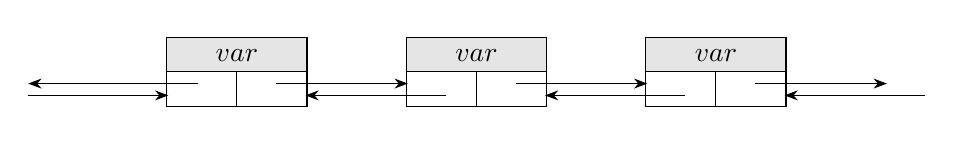
\begin{tikzpicture}[
    start chain,
    >=Stealth
    ]
    \foreach \x in {1,2,3}{
      \node (\x) [on chain] {\listNode};
    }


    % \foreach \x/\y in {1/2,2/3}{
      % \draw[->]
      % ($(\x)+(0.5,-0.15)$) -- ($(\y.180)+(0.15,-0.15)$);
      % \draw[->]
      % ($(\y)+(-0.5,-0.3)$) -- ($(\x.0)+(-0.15,-0.3)$);
      % ;
    % }

    \foreach \x in {1,2,3}{
      \draw[->]
      ($(\x)+(0.5,-0.15)$) -- ($(\x.0)+(1.15,-0.15)$);
      \draw[->]
      ($(\x)+(2.65,-0.3)$) -- ($(\x.0)+(-0.15,-0.3)$);
    }
    \draw[->]
    ($(1)+(-2.65,-0.3)$) -- ($(1.180)+(0.15,-0.3)$);
    \draw[->]
    ($(1)+(-0.5,-0.15)$) -- ($(1)+(-2.65,-0.15)$);
  \end{tikzpicture}
\end{figure}


\begin{table}
  \centering
  \begin{tabular}{l l}
    \multicolumn{2}{c}{$val$} \\
     & \\
  \end{tabular}
\end{table}


\end{document}
